\documentclass{article}
\usepackage[utf8]{inputenc}
\usepackage[T2A]{fontenc}
\usepackage[russian]{babel}
\usepackage{graphicx}
\usepackage{float}

\title{Отчет OS Лаб-6}
\author{Гаврилюк Виталий М3232}
\date{}

\begin{document}

\maketitle

\begin{figure}[H]
\centering
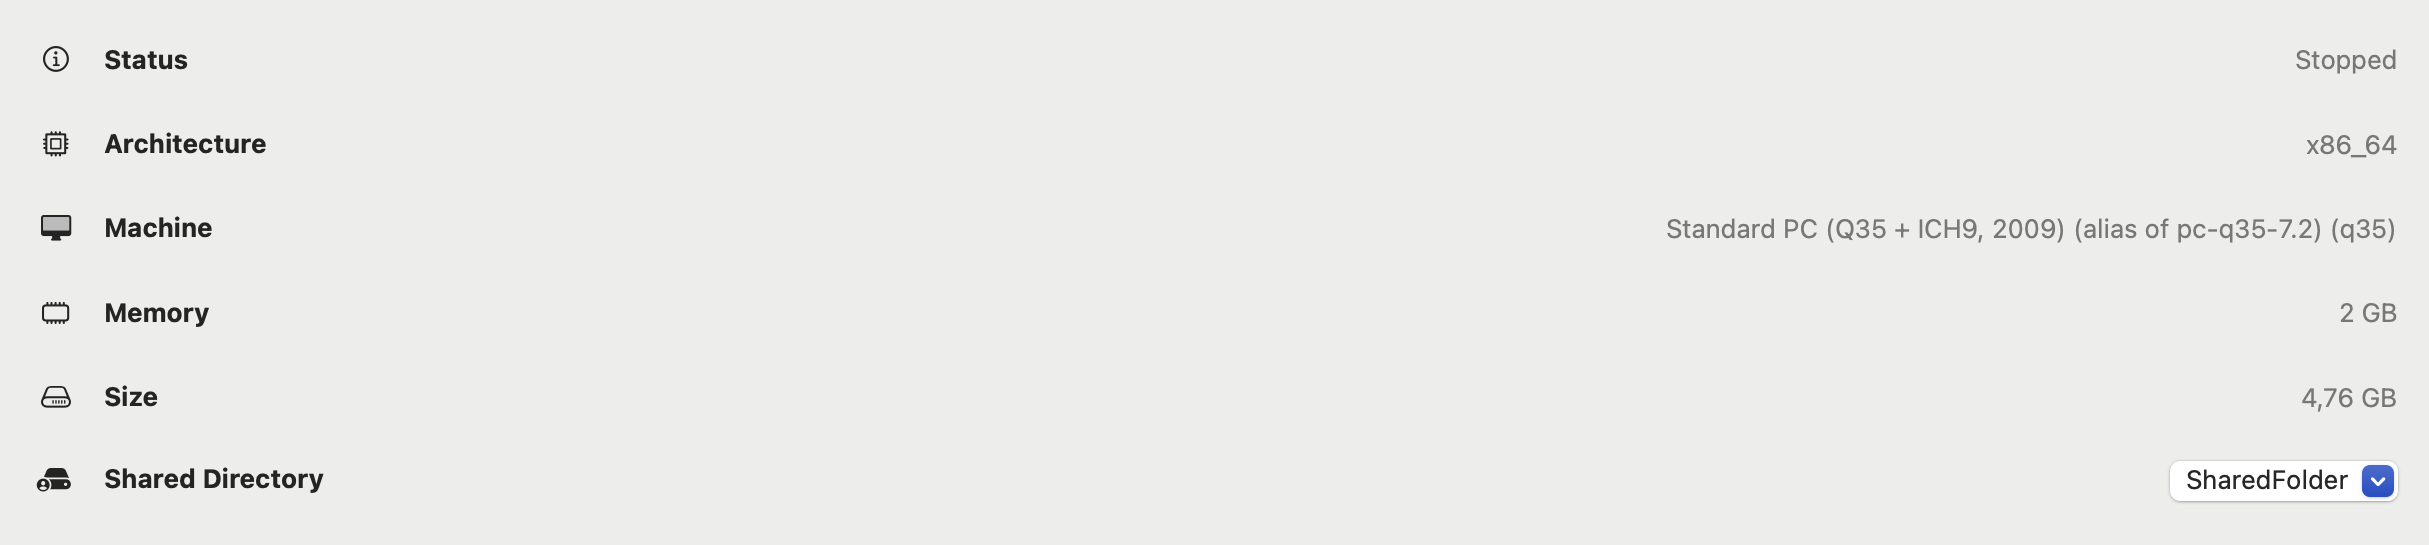
\includegraphics[width=1\textwidth]{images/1.png}
\caption{Параметры виртуальной машины}
\end{figure} 

\section*{Эксперимент 1}

\begin{figure}[H]
\centering
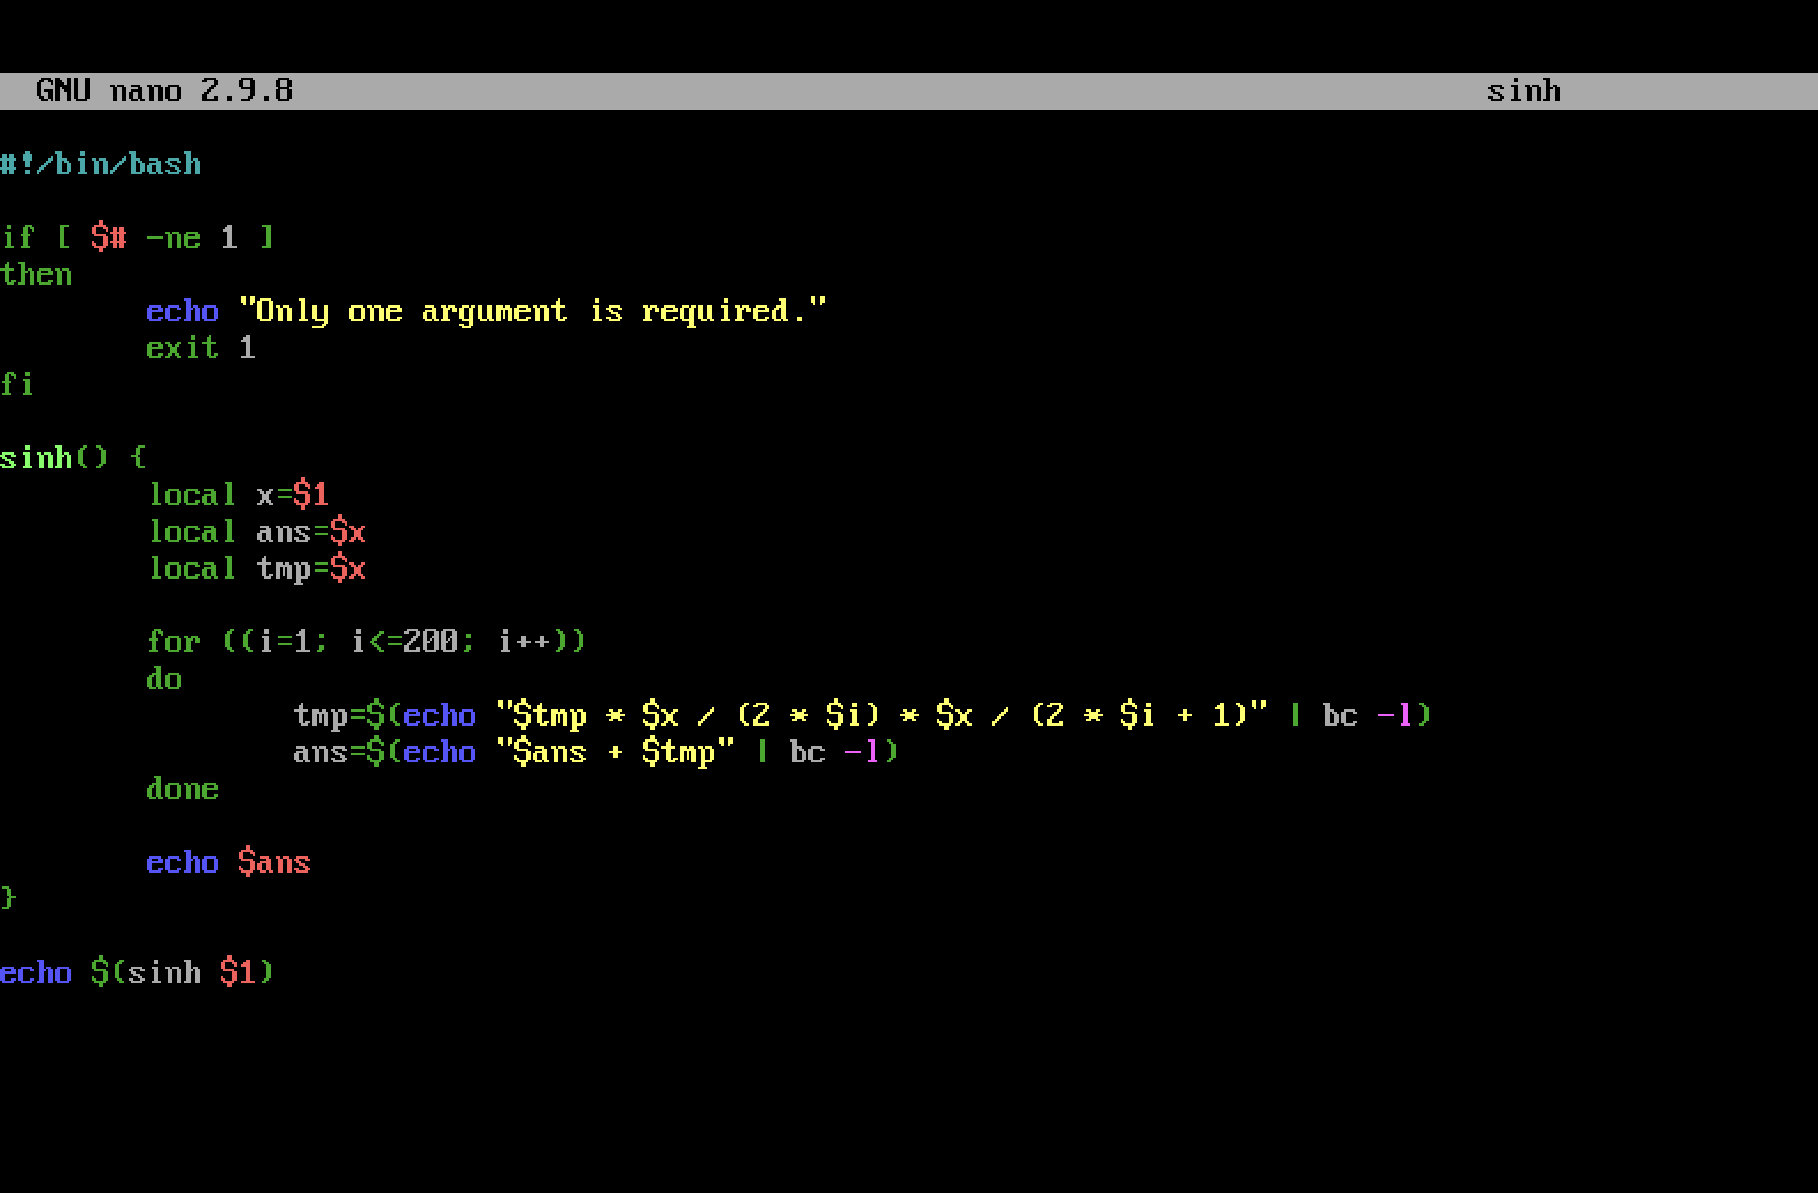
\includegraphics[width=1\textwidth]{images/2.png}
\caption{Вычислительно сложная функция (разложение рядом Маклорена)}
\end{figure} 

\begin{figure}[H]
\centering
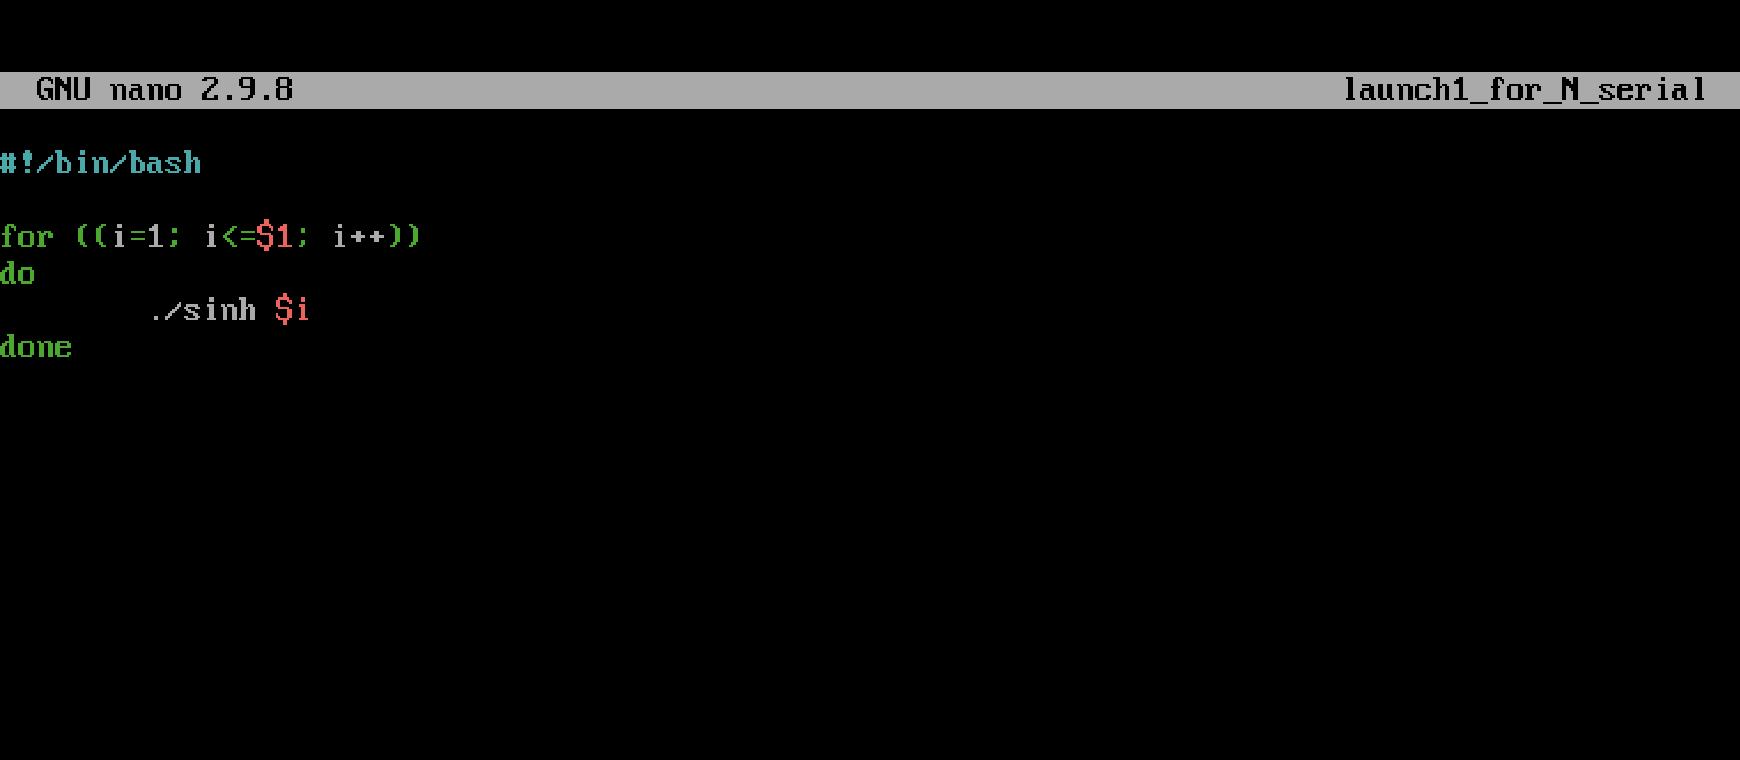
\includegraphics[width=1\textwidth]{images/3.png}
\caption{launch1-for-N-serial: запуск основного скрипта 10 раз для невилирования влияния случайных процессов}
\end{figure}

\begin{figure}[H]
\centering
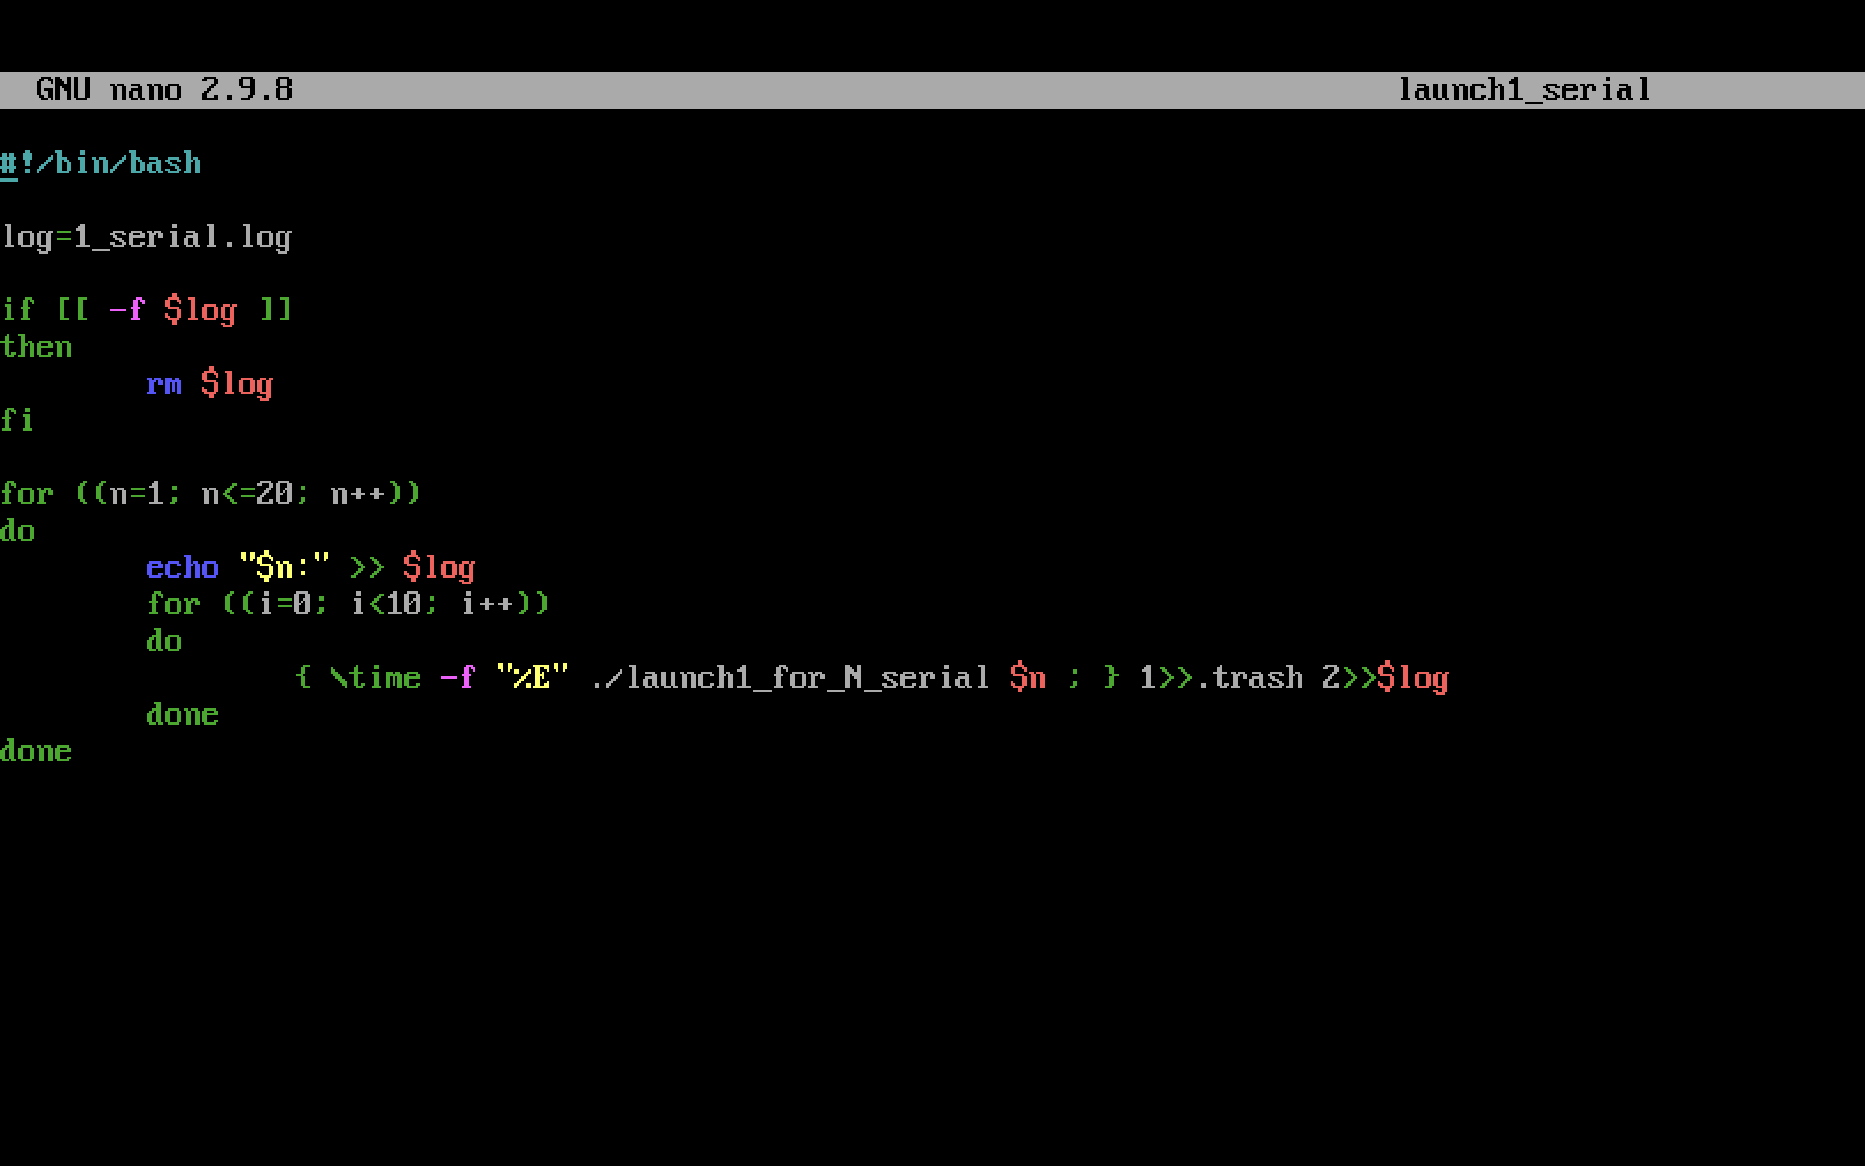
\includegraphics[width=1\textwidth]{images/4.png}
\caption{launch1-serial: запуск основного скрипта для каждого N от 1 до 20}
\end{figure}

\begin{figure}[H]
\centering
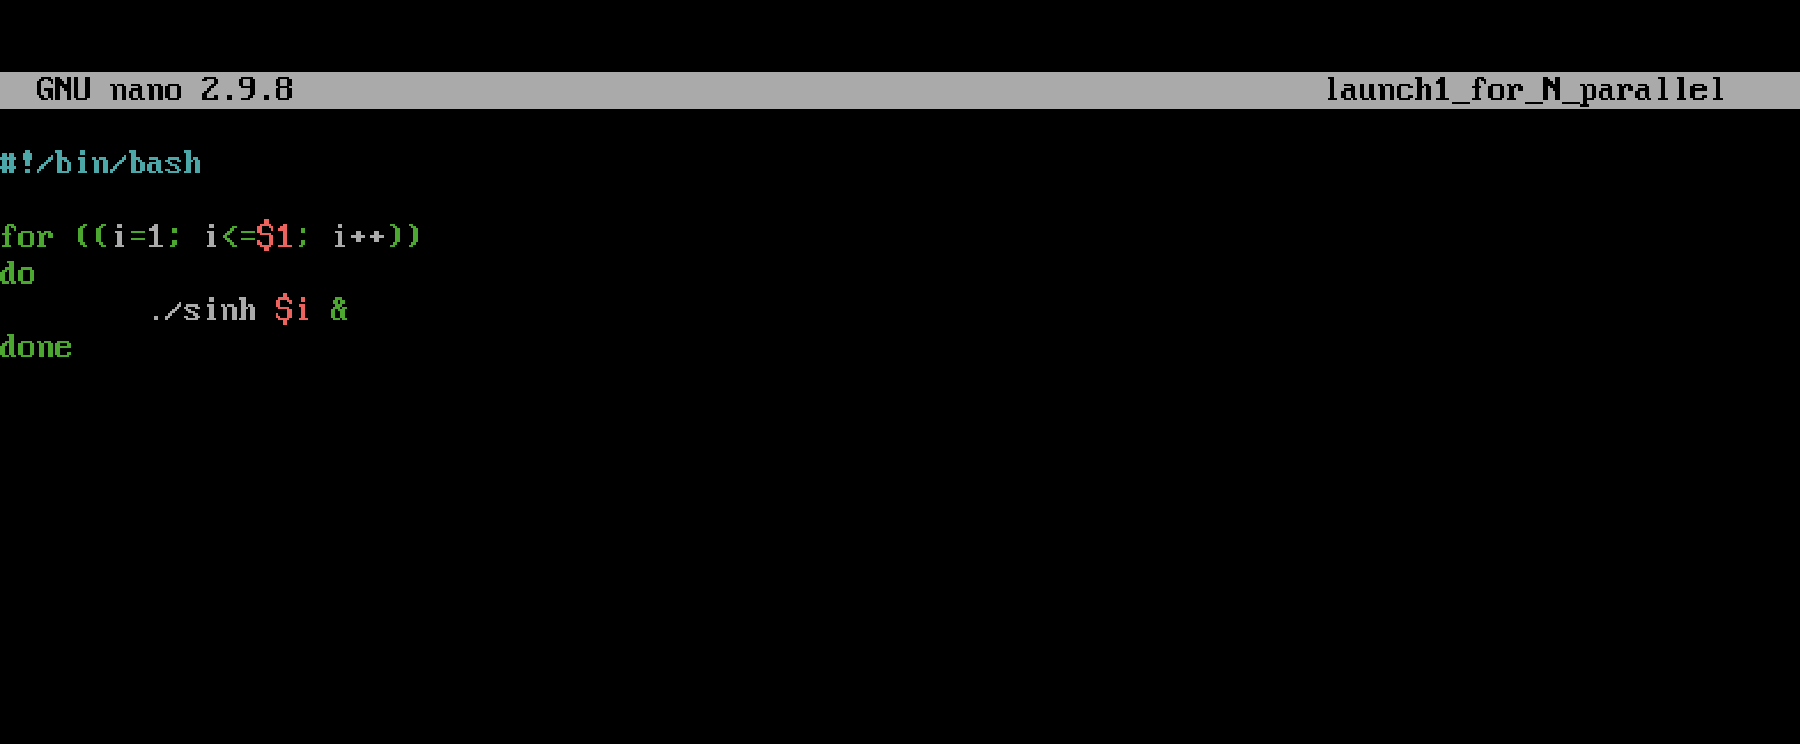
\includegraphics[width=1\textwidth]{images/7.png}
\caption{launch1-for-N-parallel: параллельный запуск основного скрипта 10 раз для невилирования влияния случайных процессов}
\end{figure}

\begin{figure}[H]
\centering
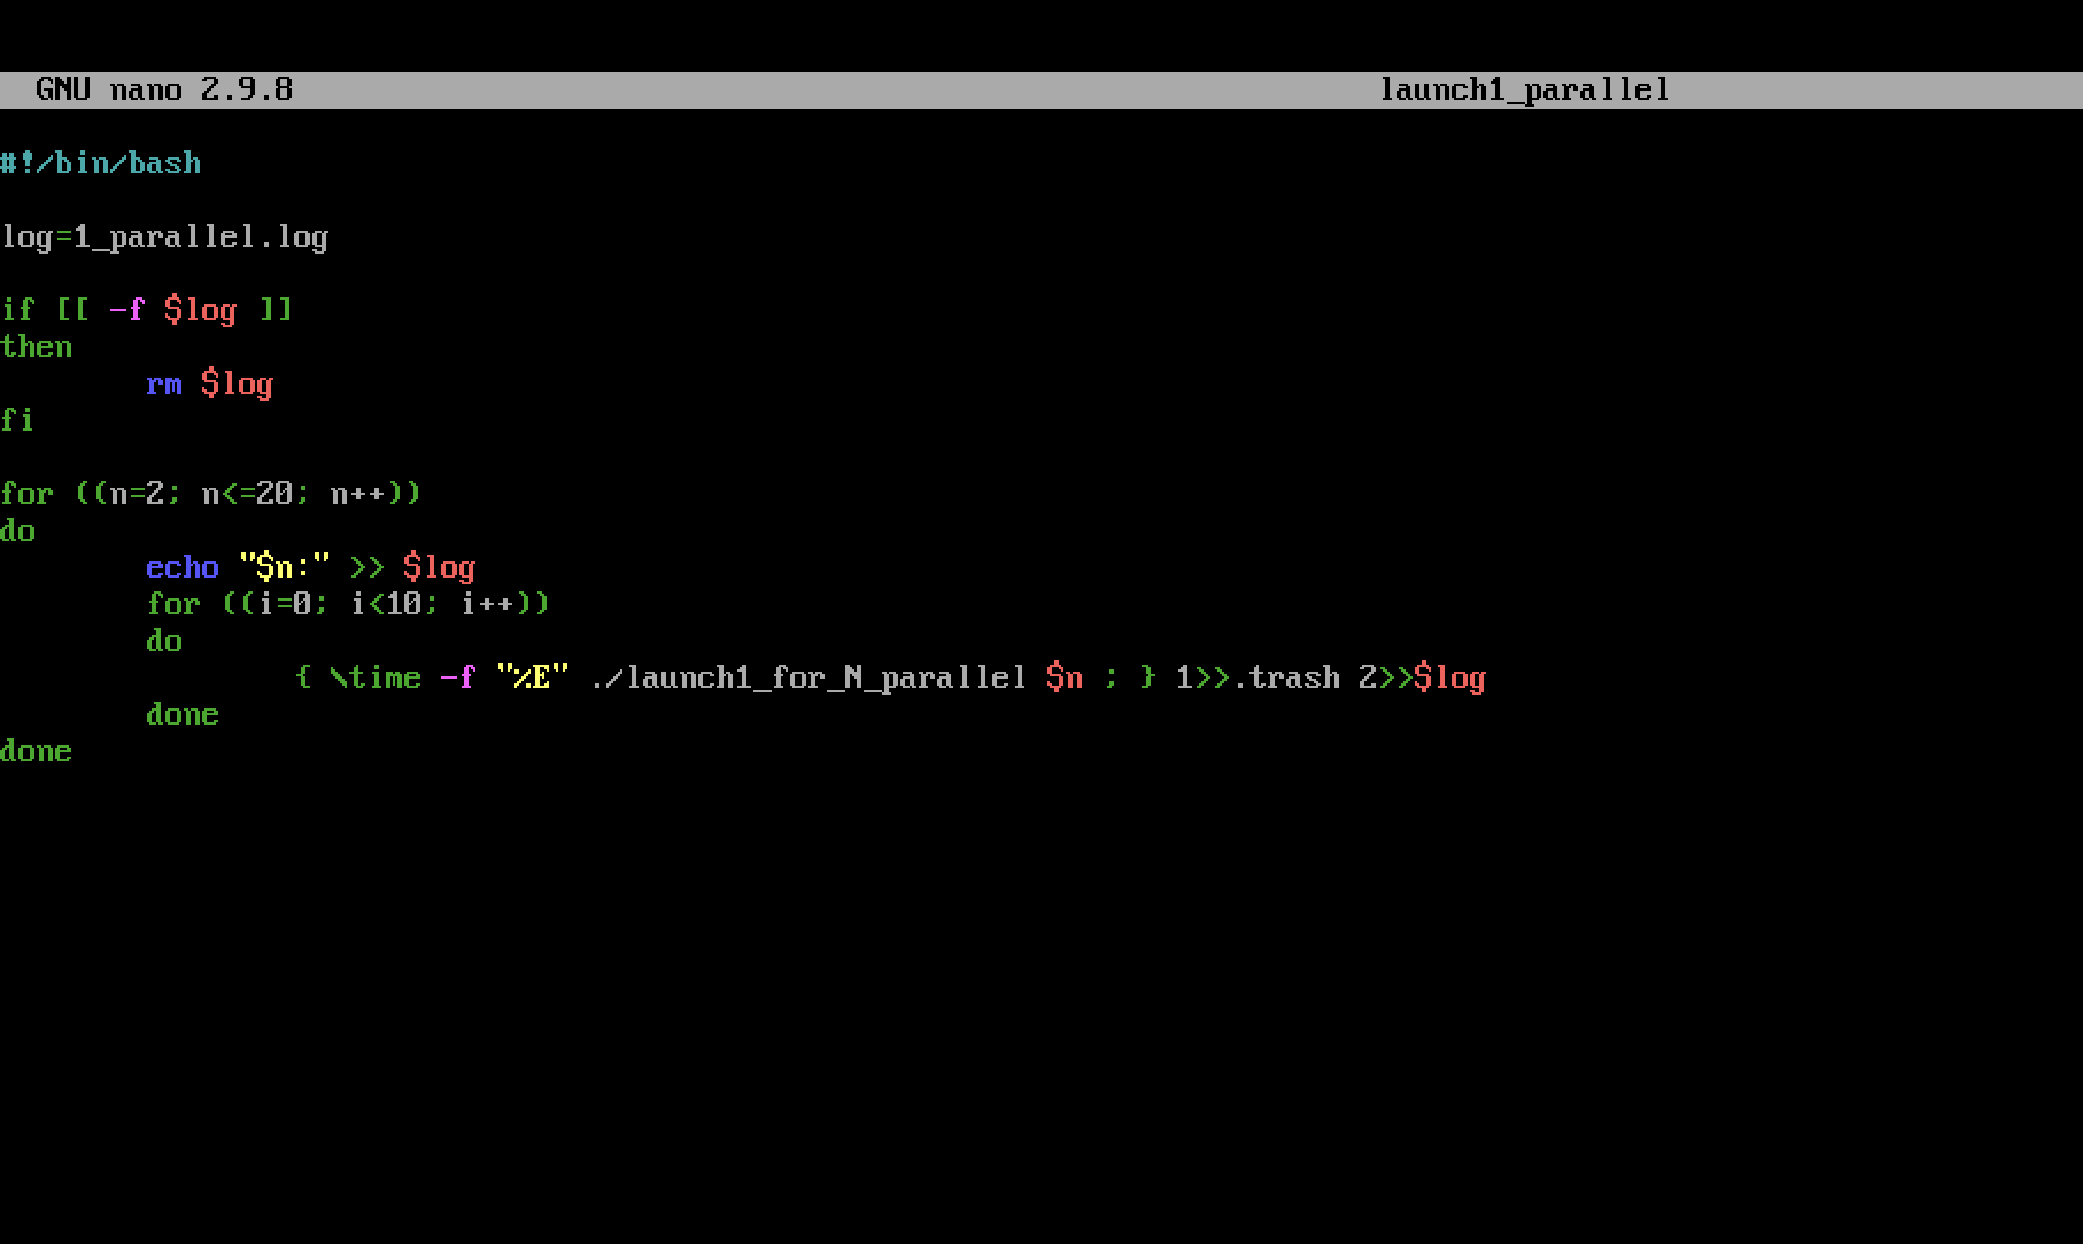
\includegraphics[width=1\textwidth]{images/8.png}
\caption{launch1-parallel: параллельный запуск основного скрипта для каждого N от 1 до 20}
\end{figure}

\begin{figure}[H]
\centering
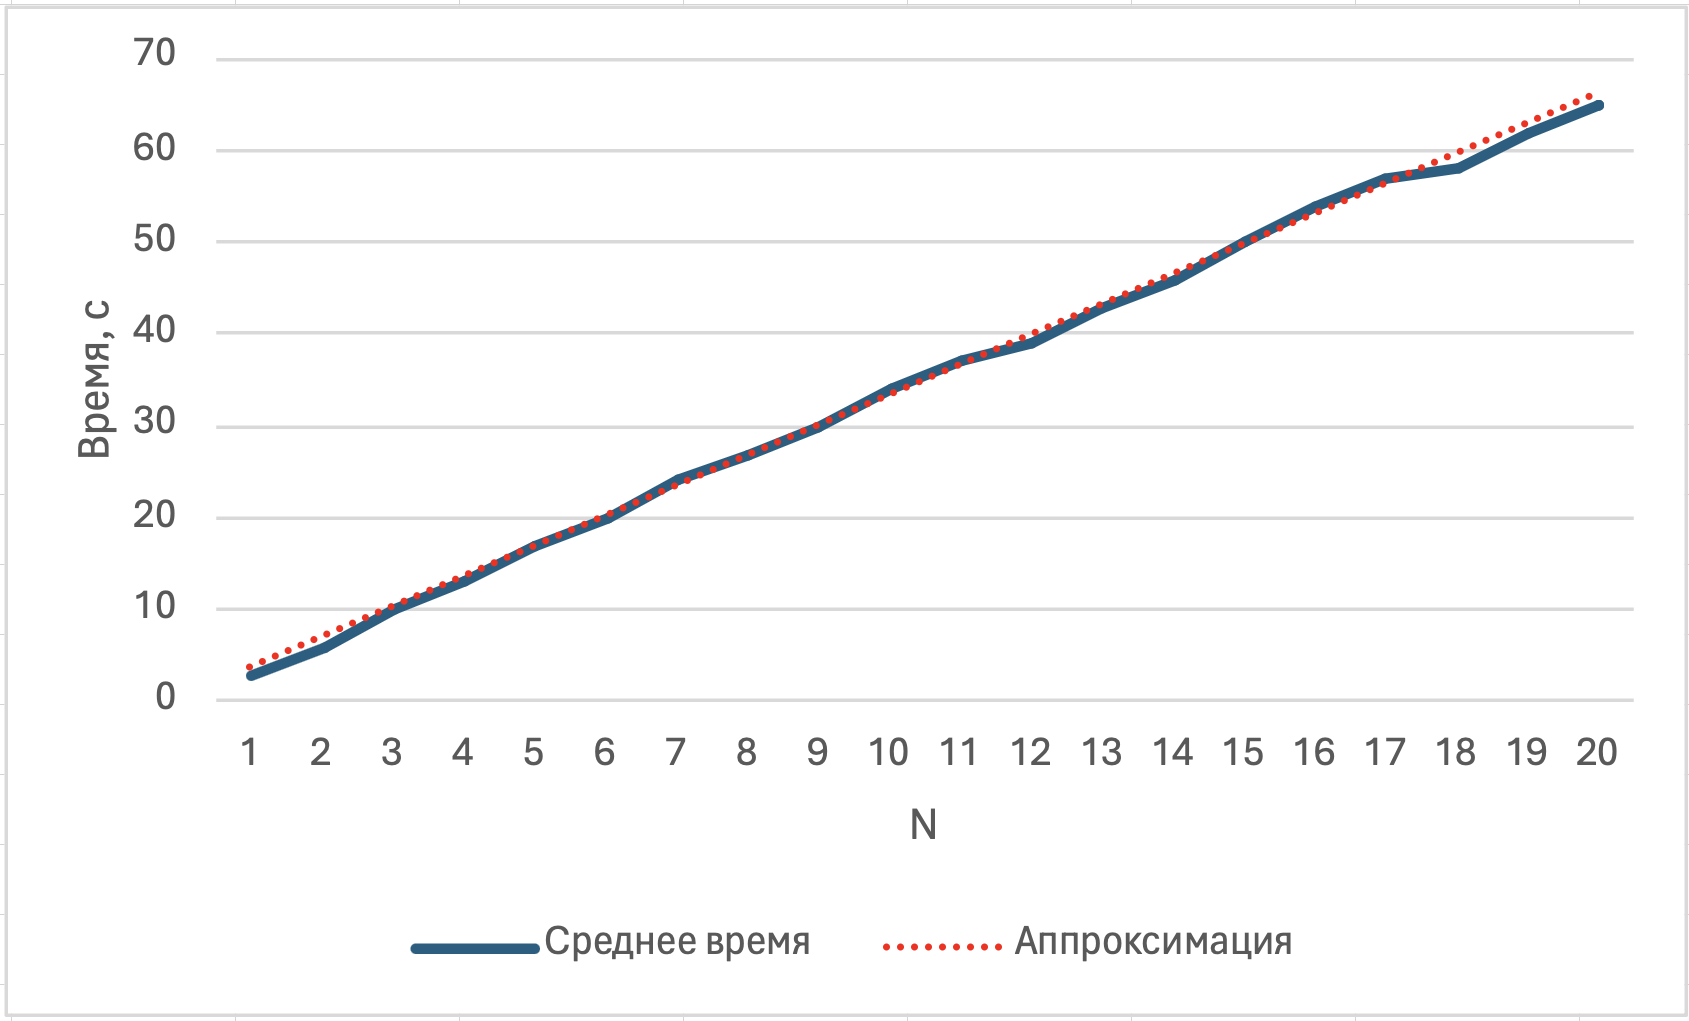
\includegraphics[width=1\textwidth]{images/5.png}
\caption{Результат последовательного выполнения кода на одном процессоре}
\end{figure}

Скрипты работают последовательно и примерно одинаково по времени, поэтому время растёт линейно.

\begin{figure}[H]
\centering
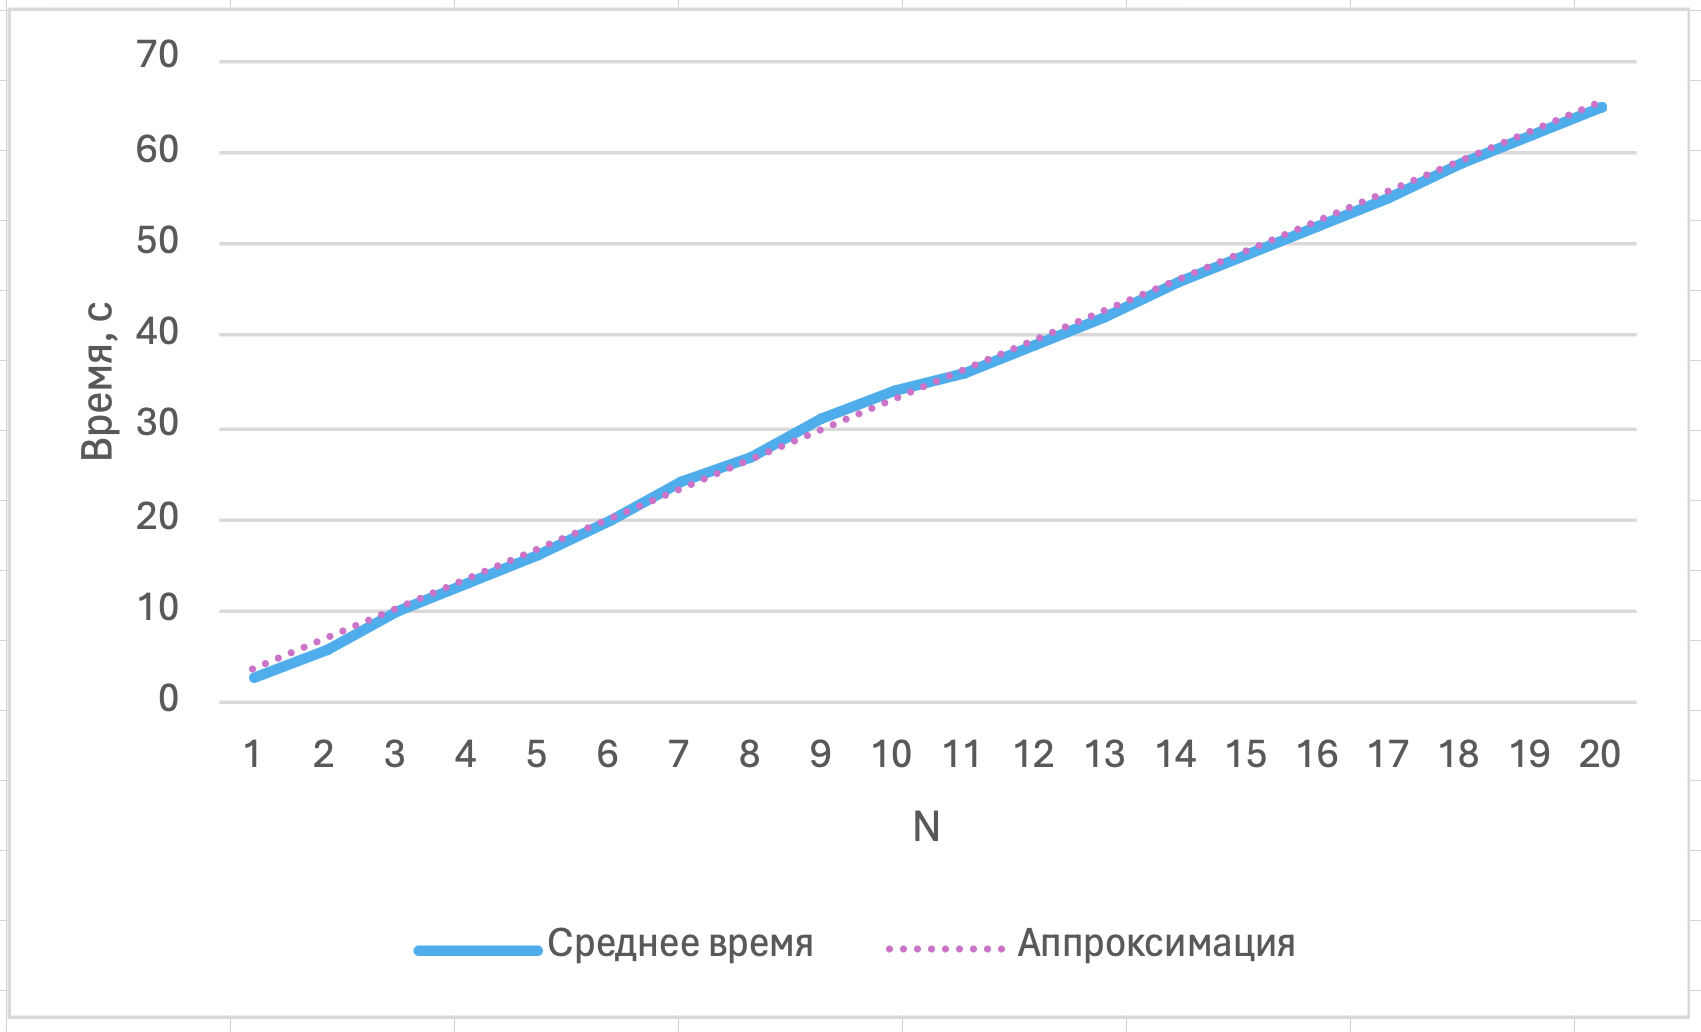
\includegraphics[width=1\textwidth]{images/6.png}
\caption{Результат параллельного выполнения кода на одном процессоре}
\end{figure}

Так как все скрипты запускаются на одном процессоре, то даже при паралельном их запуске они выполняются последовательно. Поочередно операционная система дает выполняться одному из процессов.

\begin{figure}[H]
\centering
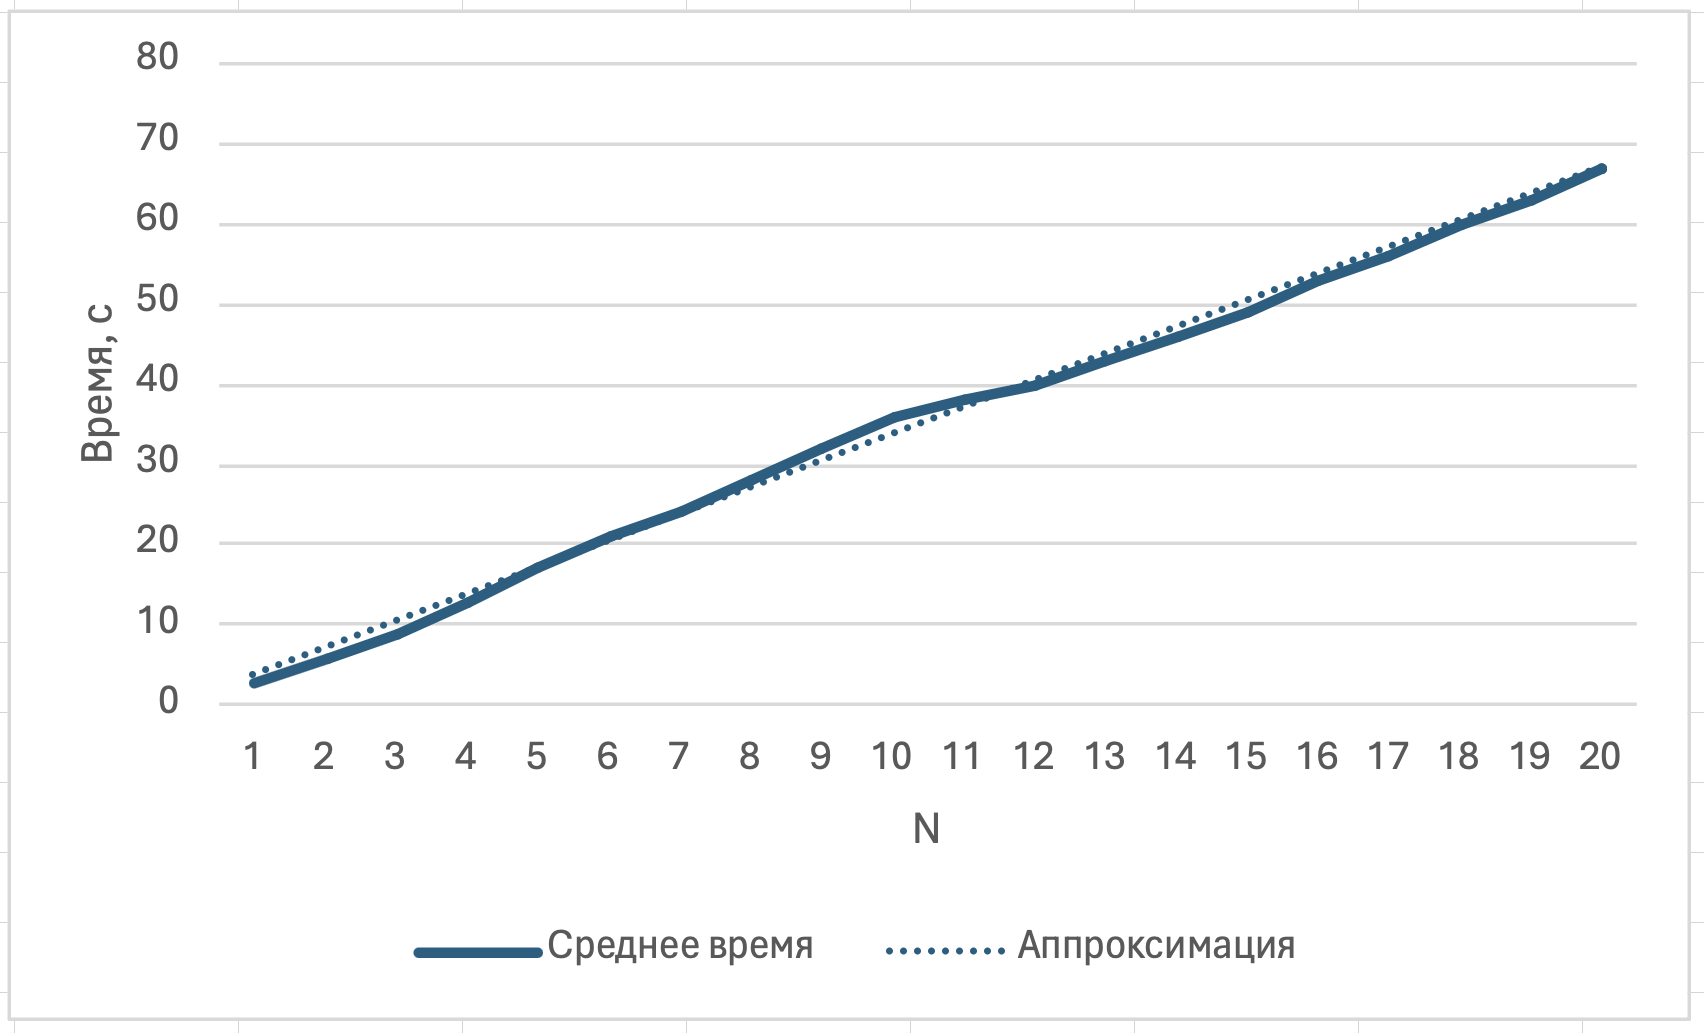
\includegraphics[width=1\textwidth]{images/9.png}
\caption{Результат последовательного выполнения кода на двух процессорах}
\end{figure}

Функция по-прежнему линейна и мало отличается от предыдущих.

\begin{figure}[H]
\centering
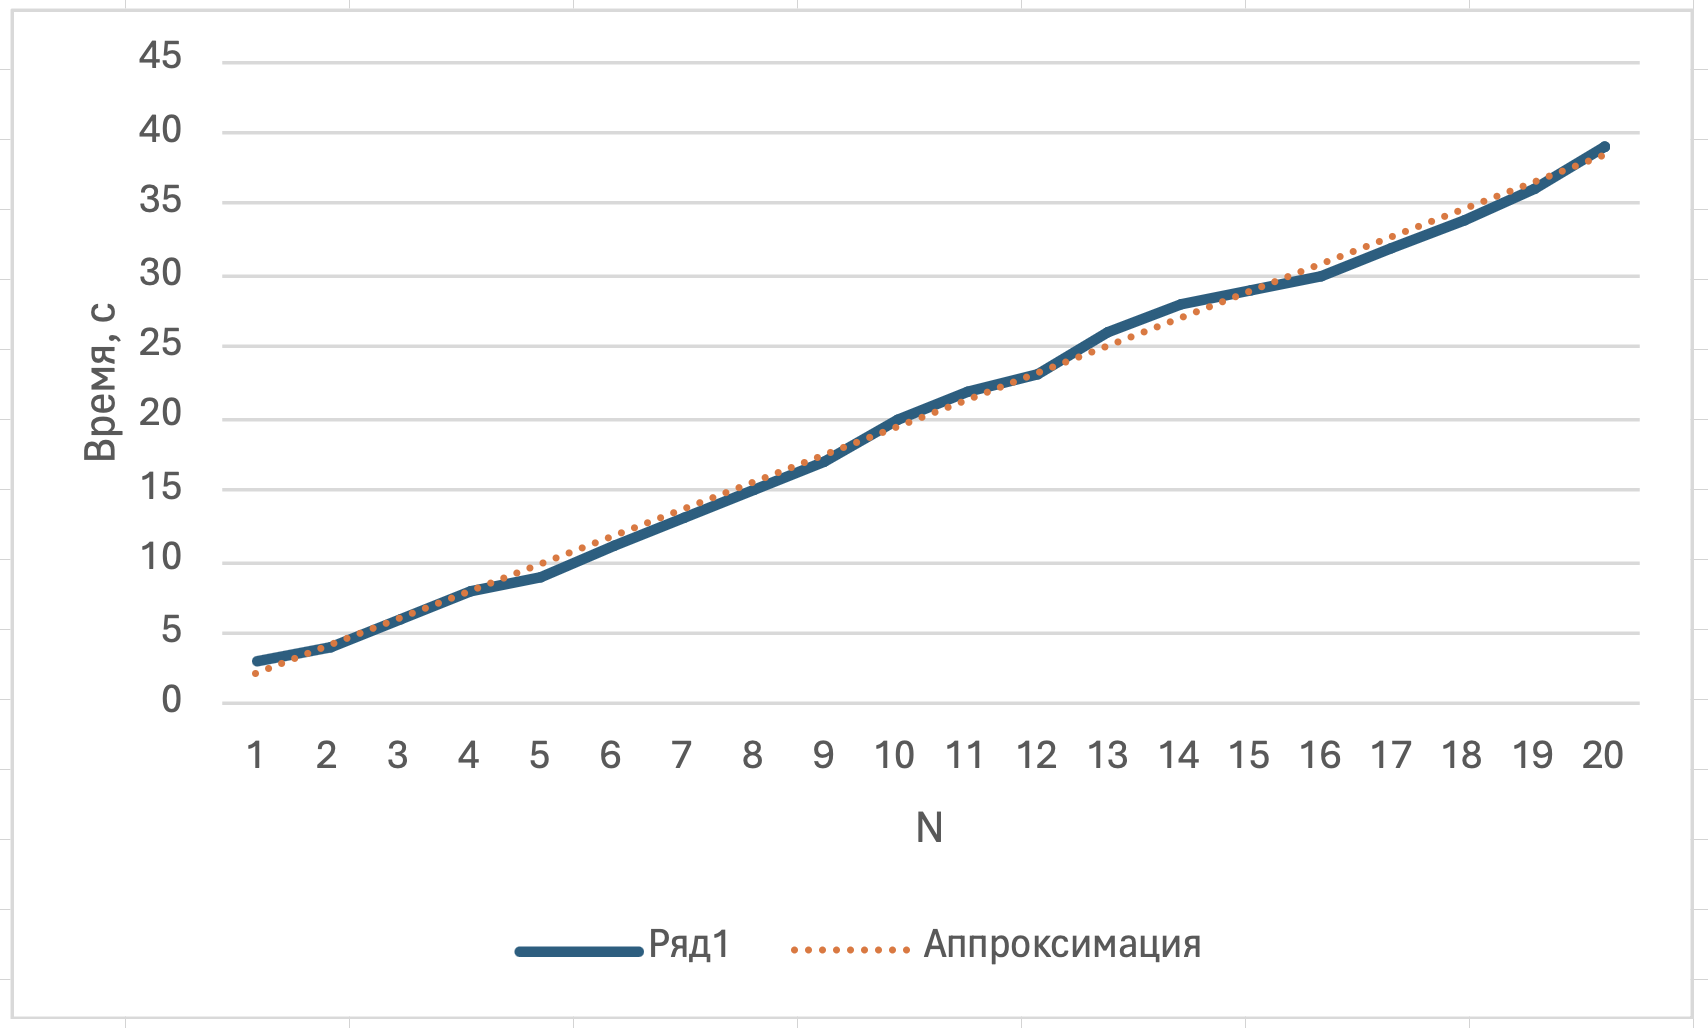
\includegraphics[width=1\textwidth]{images/10.png}
\caption{Результат параллельного выполнения кода на двух процессорах}
\end{figure}

График всё ещё линейный, но с коэфициентом почти в два раза меньше. То есть параллельное выполнение кода на двух процессорах ускоряют процесс почти в 2 раза.

\section*{Эксперимент 2}

\begin{figure}[H]
\centering
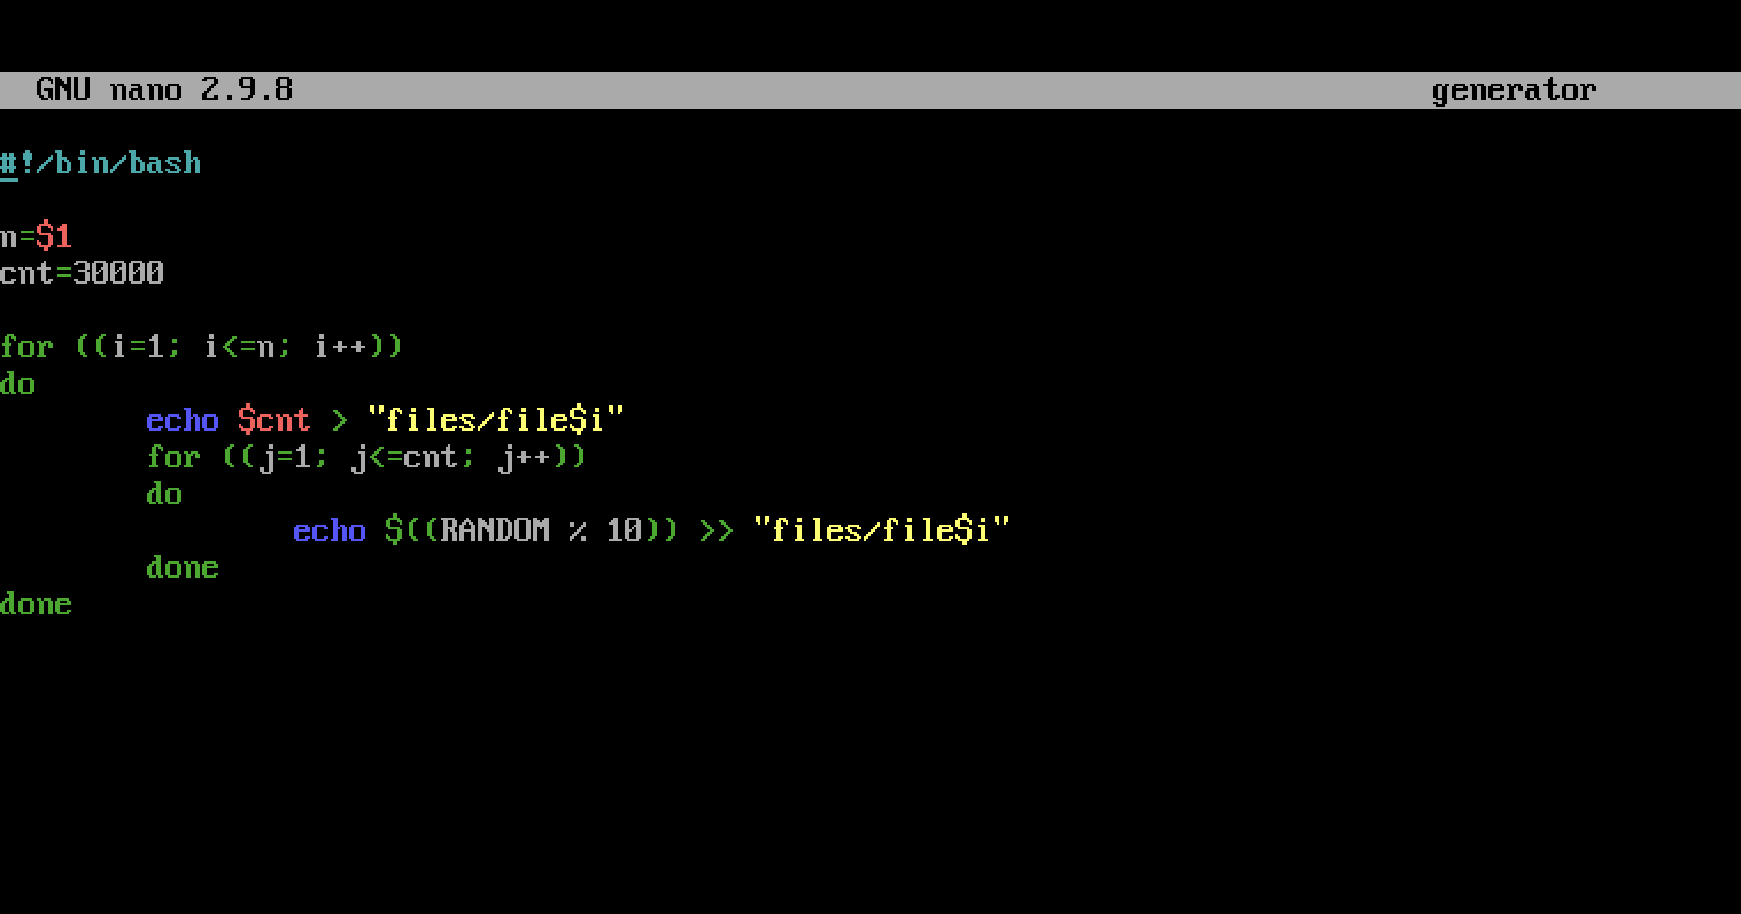
\includegraphics[width=1\textwidth]{images/11.png}
\caption{Функция с простыми вычислениями и обработкой больших массивов данных}
\end{figure} 

\begin{figure}[H]
\centering
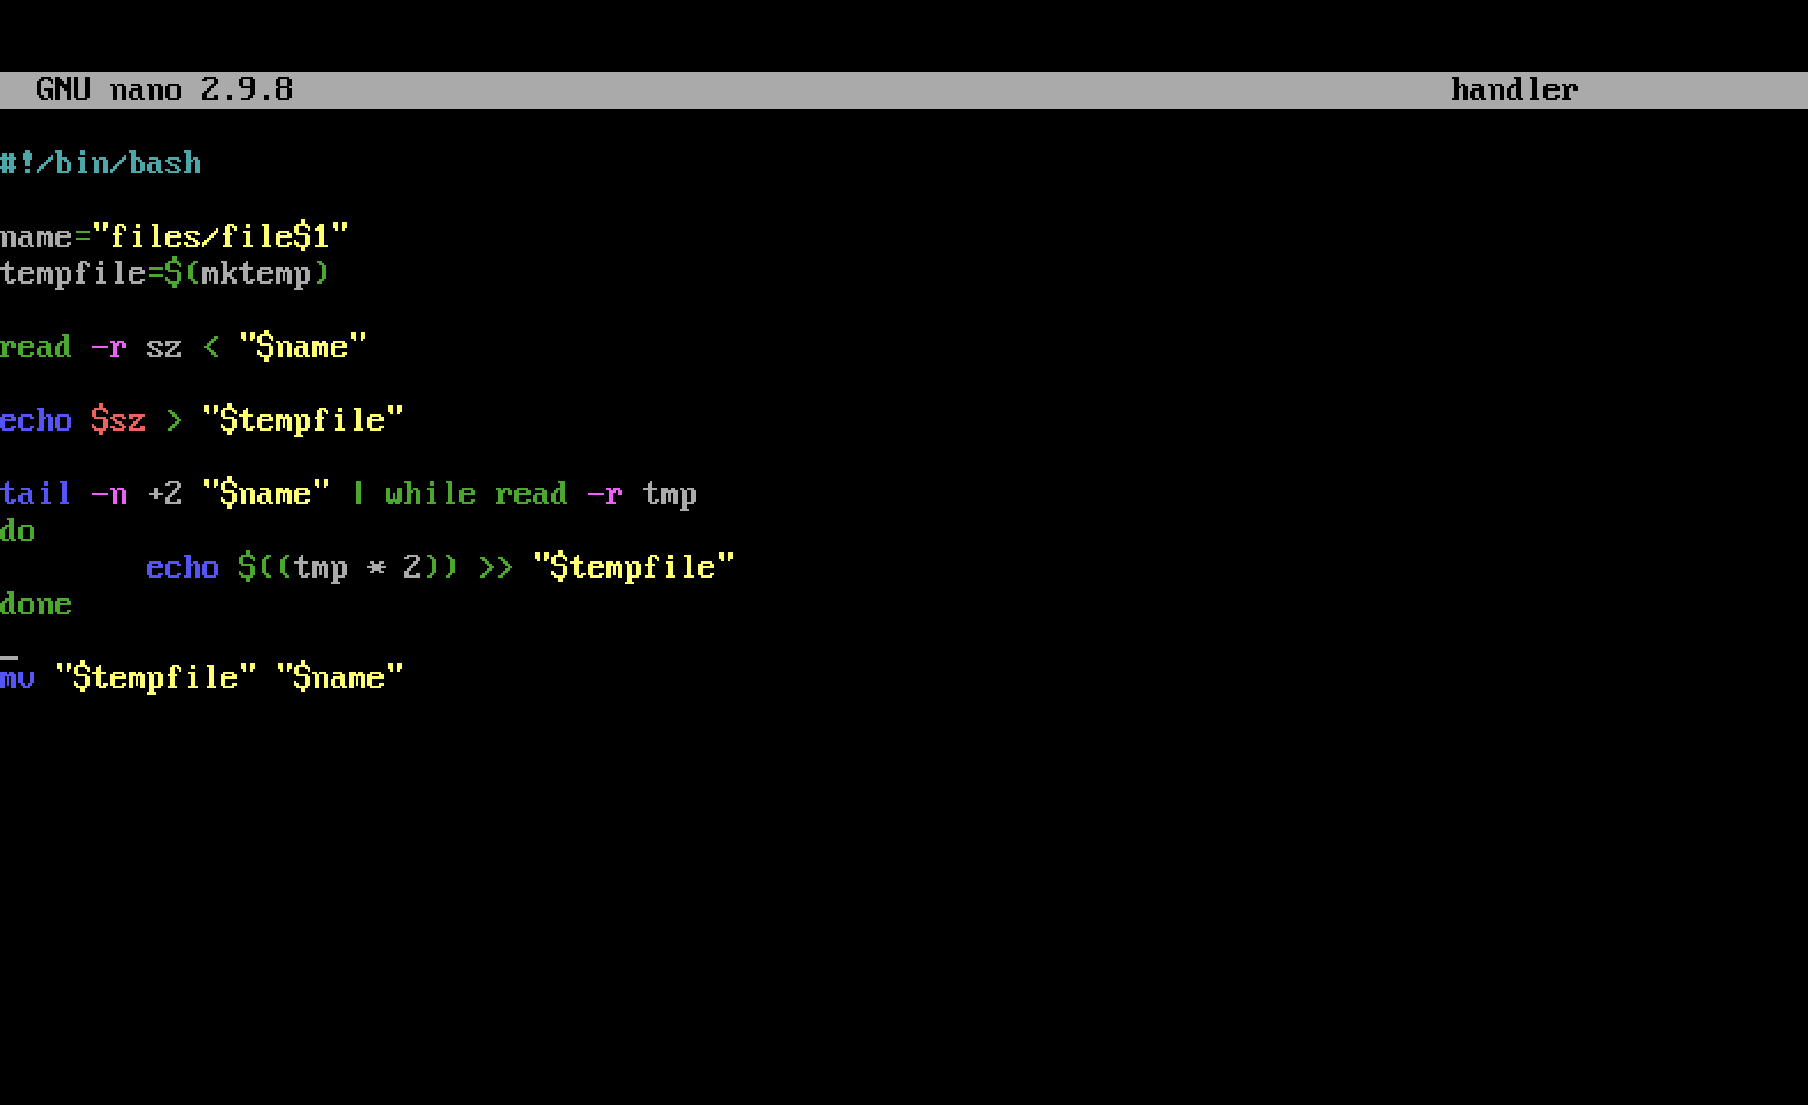
\includegraphics[width=1\textwidth]{images/12.png}
\caption{Генератор данных (используется до запуска обработчика и, поэтому, не влияет на время выполнения)}
\end{figure} 

\begin{figure}[H]
\centering
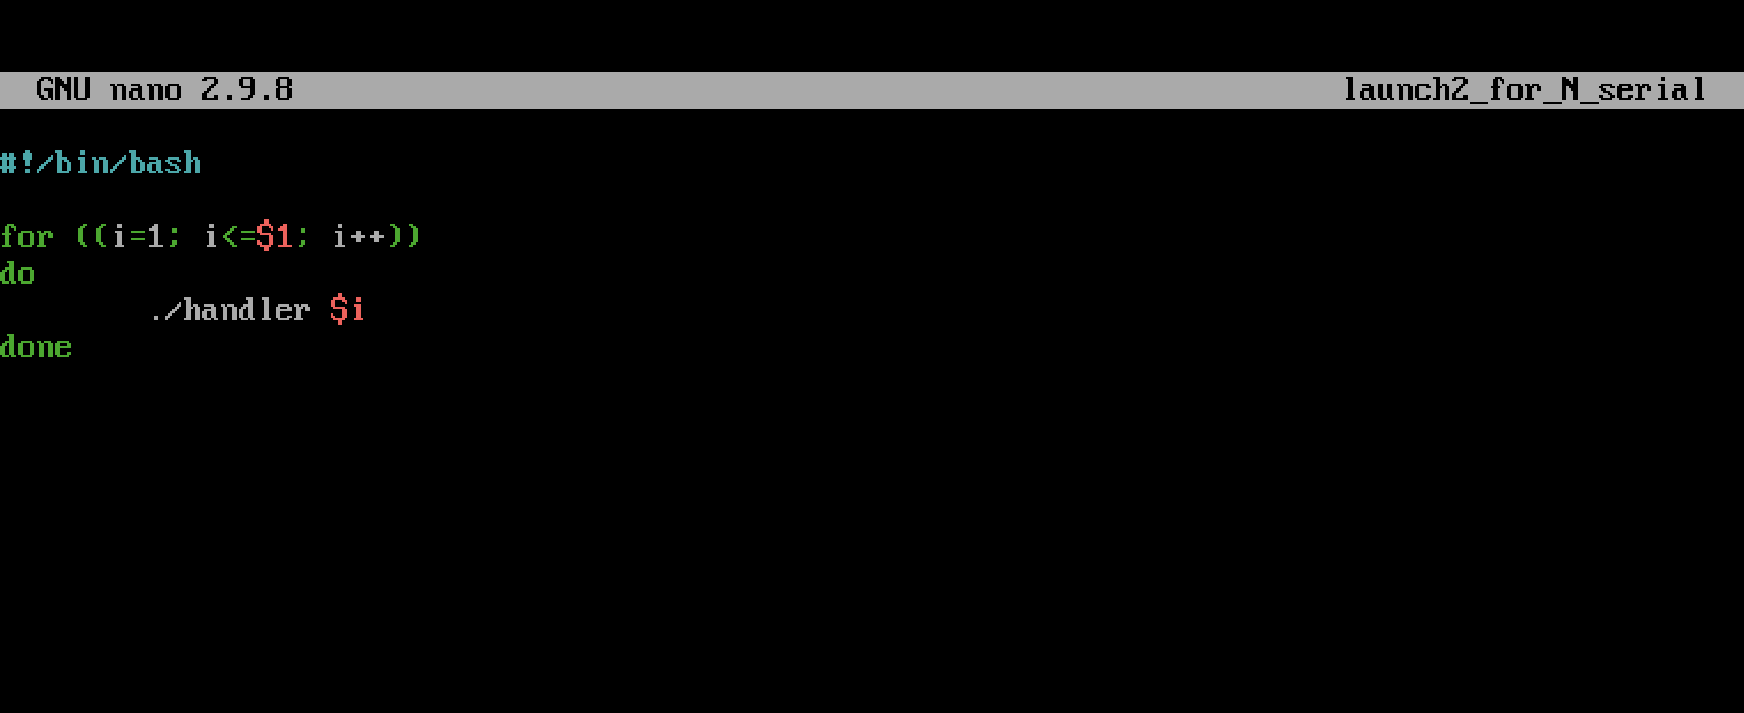
\includegraphics[width=1\textwidth]{images/13.png}
\caption{launch2-for-N-serial: запуск основного скрипта 10 раз для невилирования влияния случайных процессов}
\end{figure}

\begin{figure}[H]
\centering
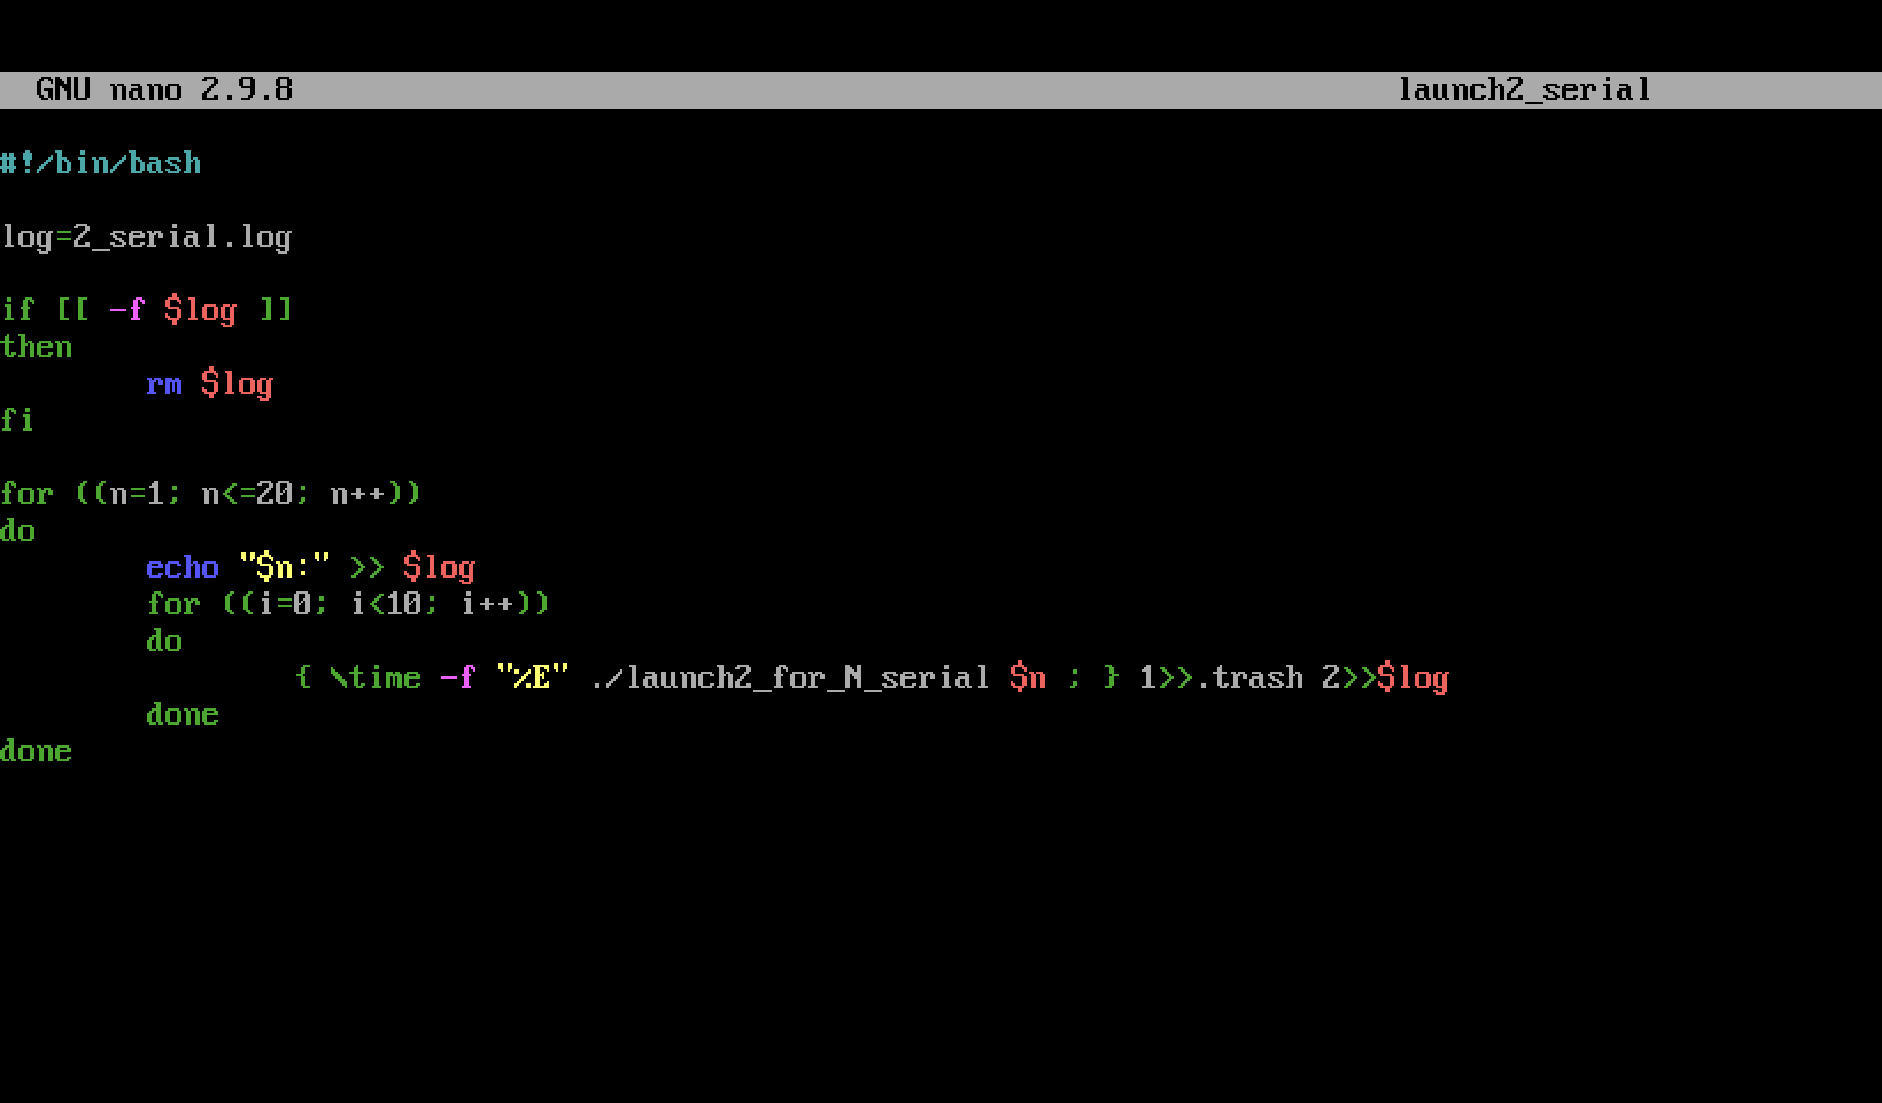
\includegraphics[width=1\textwidth]{images/14.png}
\caption{launch2-serial: запуск основного скрипта для каждого N от 1 до 20}
\end{figure}

\begin{figure}[H]
\centering
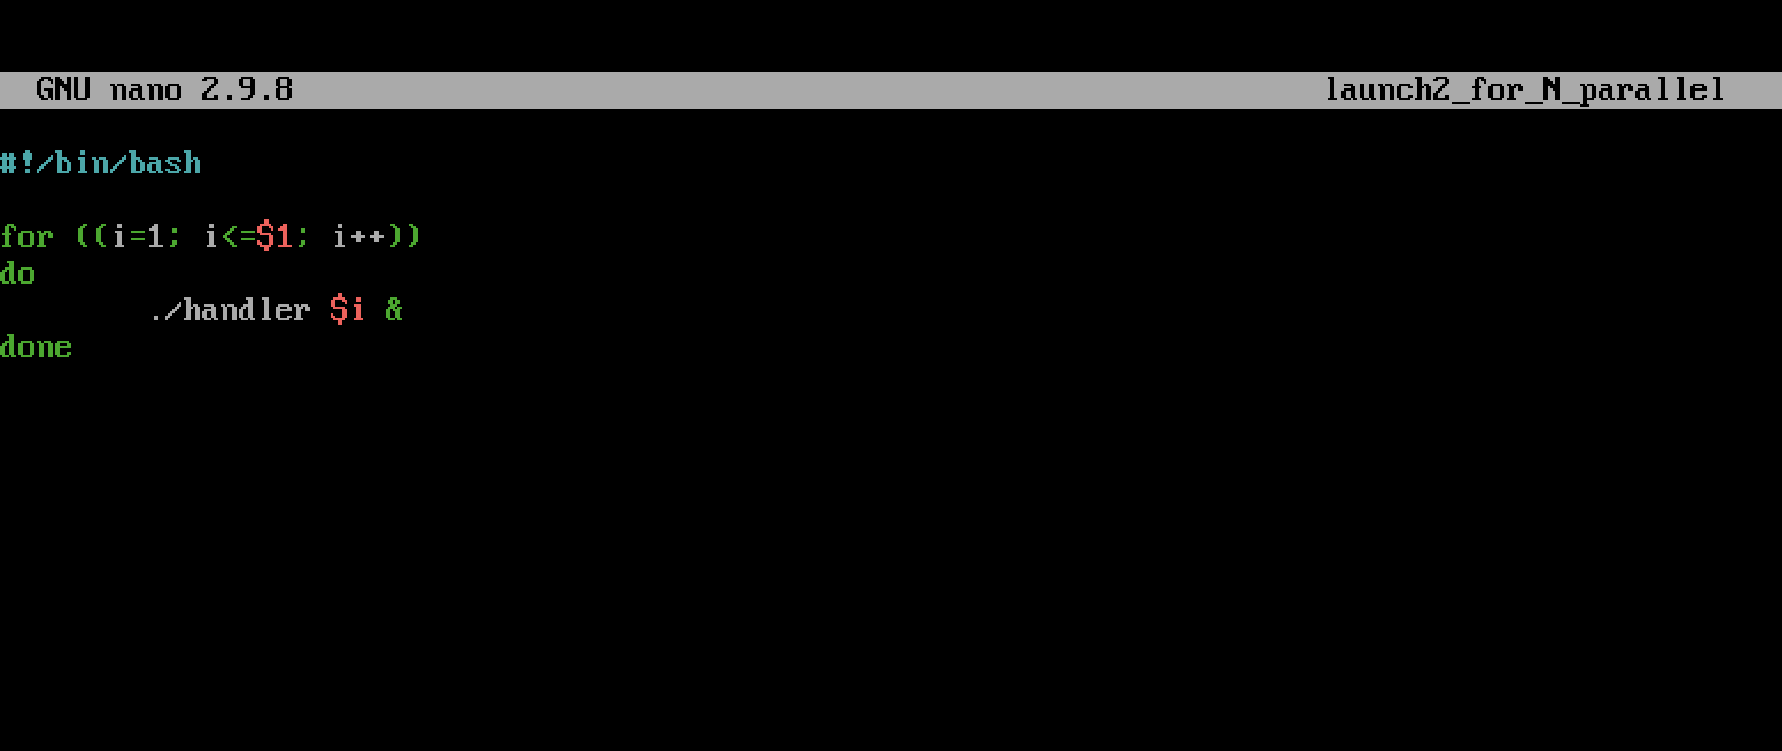
\includegraphics[width=1\textwidth]{images/15.png}
\caption{launch2-for-N-parallel: параллельный запуск основного скрипта 10 раз для невилирования влияния случайных процессов}
\end{figure}

\begin{figure}[H]
\centering
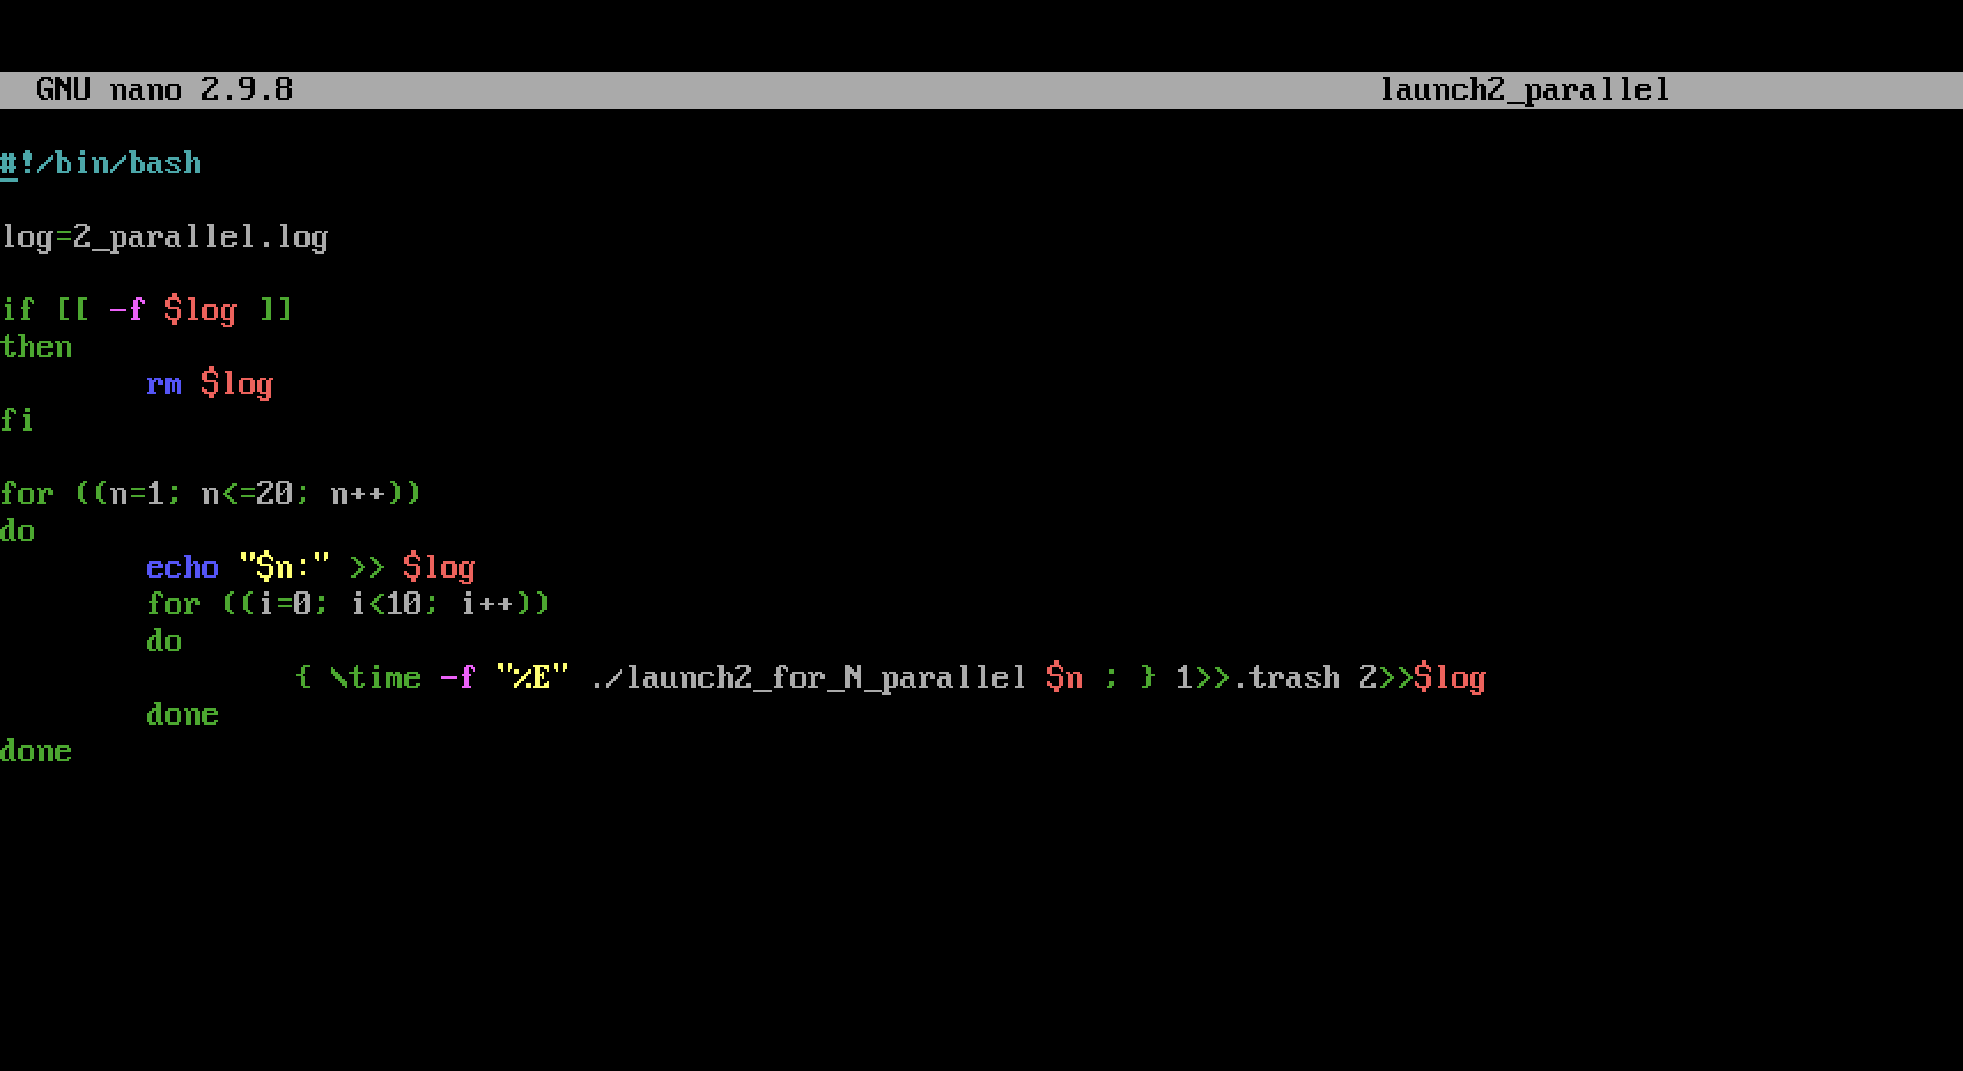
\includegraphics[width=1\textwidth]{images/16.png}
\caption{launch2-parallel: параллельный запуск основного скрипта для каждого N от 1 до 20}
\end{figure}

\begin{figure}[H]
\centering
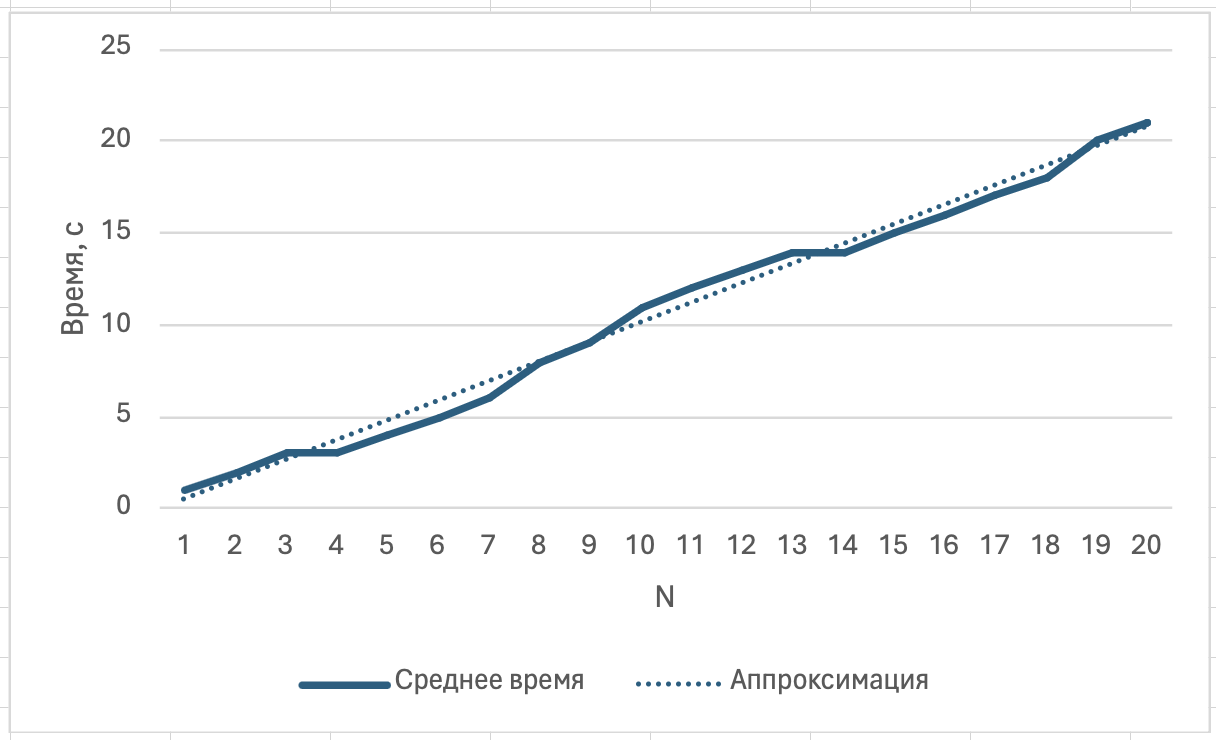
\includegraphics[width=1\textwidth]{images/17.png}
\caption{Результат последовательного выполнения кода на одном процессоре}
\end{figure}

\begin{figure}[H]
\centering
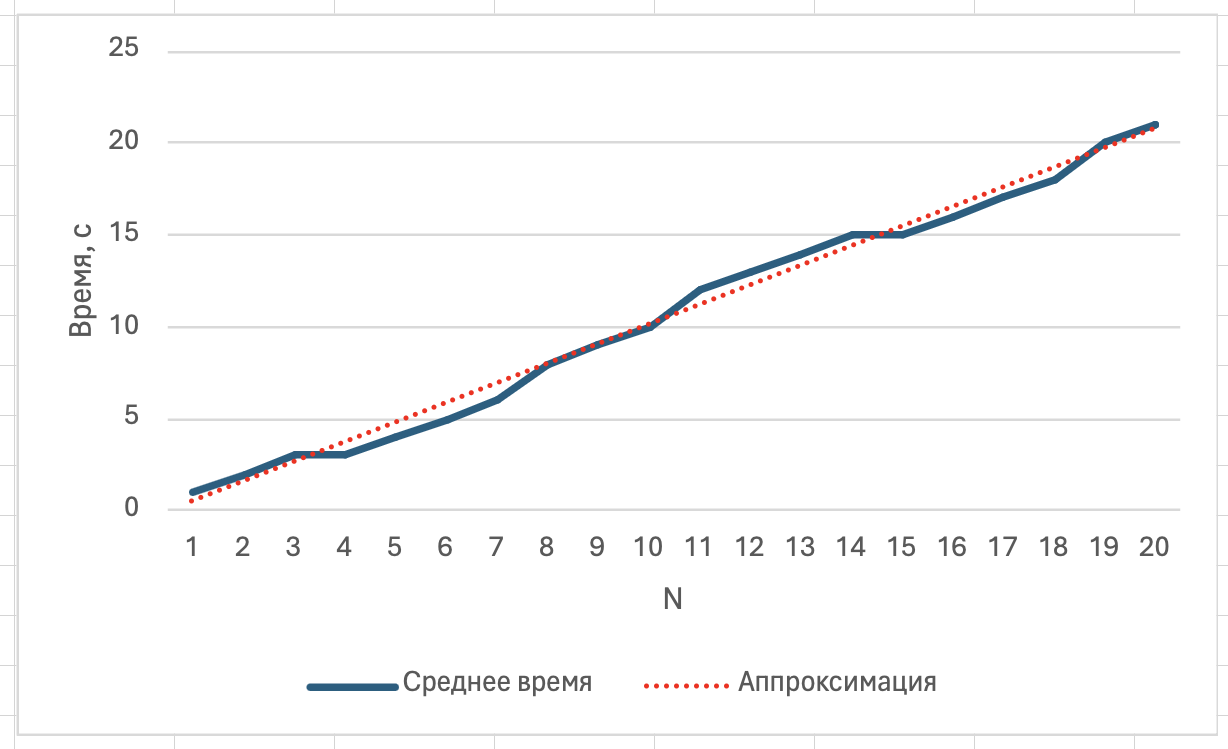
\includegraphics[width=1\textwidth]{images/18.png}
\caption{Результат параллельного выполнения кода на одном процессоре}
\end{figure}

\begin{figure}[H]
\centering
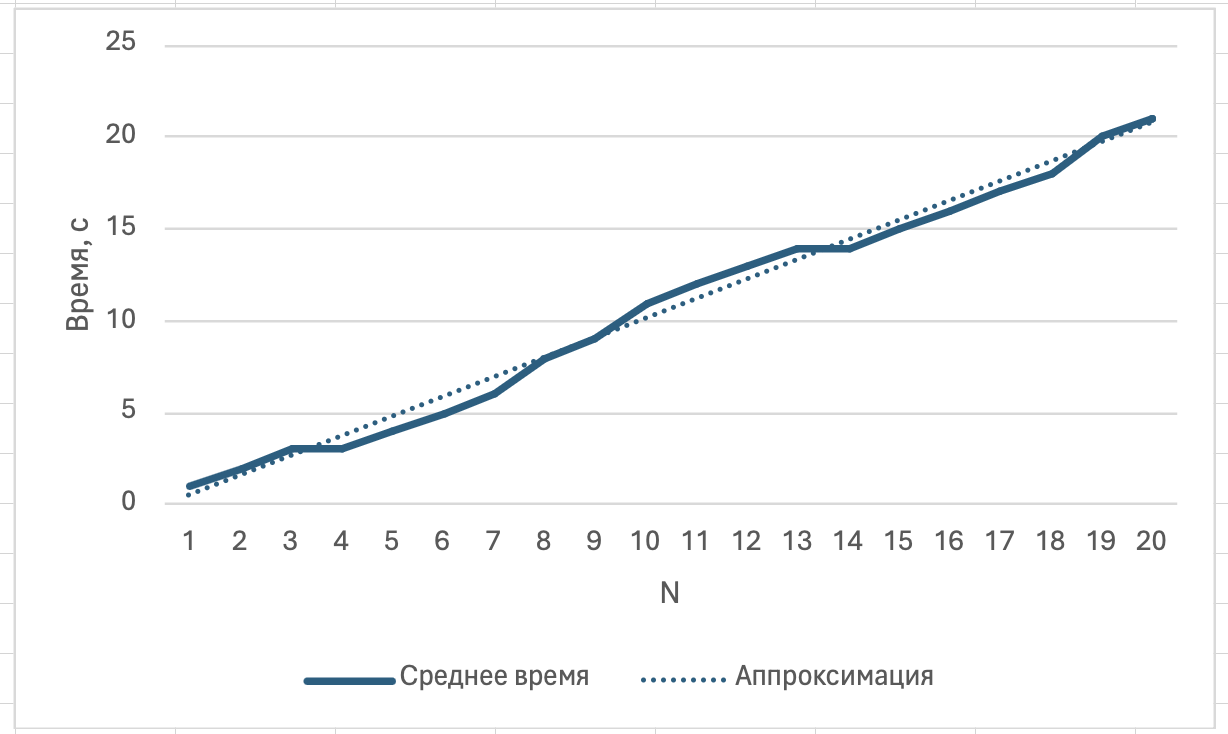
\includegraphics[width=1\textwidth]{images/19.png}
\caption{Результат последовательного выполнения кода на двух процессорах}
\end{figure}

\begin{figure}[H]
\centering
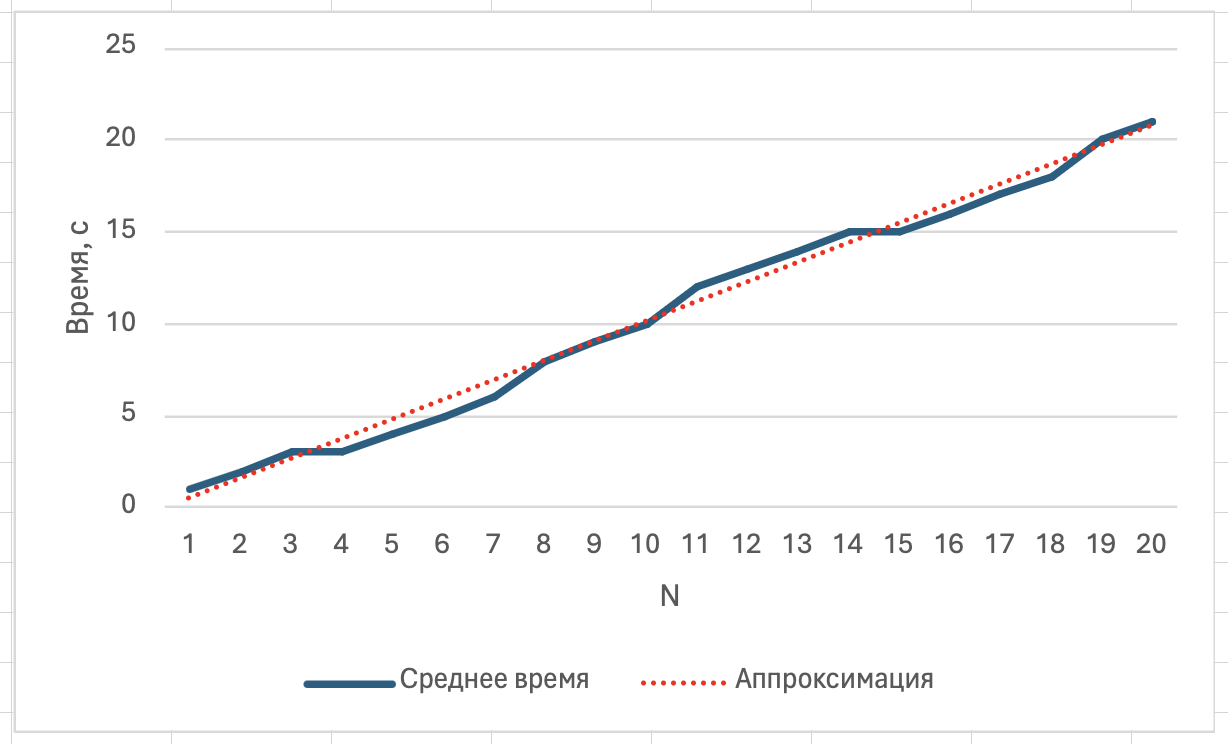
\includegraphics[width=1\textwidth]{images/20.png}
\caption{Результат параллельного выполнения кода на двух процессорах}
\end{figure}


Вывод: во всех четырёх случаях -- линейный рост, в первых трех коэфициент примерно одинаковый, в четвёртом почти в 2 раза меньше (параллельный запуск на 2 двух процессорах)


\end{document}